% ! TeX program = lualatex
\documentclass[a4paper,11pt]{article} 
% packages
\usepackage{censor}
\StopCensoring
\usepackage{fontspec}
\setmainfont{EB Garamond}
% for tironian et fallback
% % \directlua{luaotfload.add_fallback
% % ("emojifallback",
% %      {"Noto Serif:mode=harf"}
% % )}
% % \setmainfont{EB Garamond}[RawFeature={fallback=emojifallback}]

\setmonofont[Scale=MatchLowercase]{Deja Vu Sans Mono}
\usepackage[a4paper,left=2cm,right=2cm,top=\dimexpr15mm+1.5\baselineskip,bottom=2cm]{geometry}
\setlength{\parindent}{0pt}

\usepackage{fancyhdr}       % Headers and footers 
\fancyhead[R]{\normalfont \leftmark}
\fancyhead[L]{}
\pagestyle{fancy}

\usepackage{microtype}      % Slightly tweak font spacing for aesthetics
\usepackage[english]{babel} % Language hyphenation and typographical rules
\usepackage{xcolor}
\definecolor{linkblue}{RGB}{0, 64, 128}
\usepackage[final, colorlinks = false, urlcolor = linkblue]{hyperref} 
% \newcommand{\secref}[1]{\textbf{§~\nameref{#1}}}
\newcommand{\secref}[1]{\textbf{§\ref{#1}~\nameref{#1}}}

\usepackage[most]{tcolorbox}
\usepackage{changepage}     % adjust margins on the fly
\usepackage{amsmath,amssymb}

\usepackage{minted}
\usemintedstyle{algol_nu}

\usepackage{pgfplots}
\pgfplotsset{width=\textwidth,compat=1.9}

\usepackage{caption}
\newenvironment{code}{\captionsetup{type=listing}}{}
\captionsetup[listing]{skip=0pt}
\setlength{\abovecaptionskip}{5pt}
\setlength{\belowcaptionskip}{5pt}

\usepackage[yyyymmdd]{datetime}
\renewcommand{\dateseparator}{--}

\usepackage{enumitem}

\usepackage{titlesec}

\author{Andrew Hayes}

\begin{document}
\begin{titlepage}
    \begin{center}
        \hrule
        \vspace*{0.6cm}
        \Huge \textsc{cs4423}
        \vspace*{0.6cm}
        \hrule
        \LARGE
       \vspace{0.5cm}
       Networks
       \vspace{0.5cm}
       \hrule

       \vfill

       \hrule
        \begin{minipage}{0.495\textwidth} 
            \vspace{0.4em}
            \raggedright
            \normalsize 
            \begin{tabular}{@{}l l}
                Name: & Andrew Hayes \\
                Student ID: & 21321503 \\
                E-mail: & \href{mailto://a.hayes18@universityofgalway.ie}{a.hayes18@universityofgalway.ie} \\
            \end{tabular}
        \end{minipage}
        \begin{minipage}{0.495\textwidth} 
            \raggedleft
            \vspace*{0.8cm}
            \Large
            \today
            \vspace*{0.6cm}
        \end{minipage}
        \medskip\hrule 
    \end{center}
\end{titlepage}

\pagenumbering{roman}
\newpage
\tableofcontents
\newpage
\setcounter{page}{1}
\pagenumbering{arabic}

\section{Introduction}
\textbf{CS4423 Networks} is a Semester 2 module on \textbf{Network Science}.
Modern societies are in many ways highly connected.
Certain aspects of this phenomenon are frequently described as \textbf{networks}.
CS4423 is an introduction to this emerging interdisciplinary subject.
We'll cover several major topics in this module, including:
\begin{itemize}
    \item   Graphs \& Graph Theory,  and how they relate to networks;
    \item   Representations of networks, including as matrices;
    \item   Computing with networks, using \mintinline{python}{networkx} in Python;
    \item   Centrality measures;
    \item   Random graphs;
    \item   Small worlds;
    \item   Models of growing graphs;
\end{itemize}

Lecture notes \& assignments will come in the form of Jupyter notebooks, which allows us to include interactive Python code with the text.

\subsection{Lecturer Contact Information}
\begin{itemize}
    \item   Name: Dr Niall Madden.
    \item   School of Mathematical \& Statistical Sciences, University of Galway.
    \item   Office: Room ADB-1013, Arás de Brún.
    \item   E-mail: \href{mailto://niall.madden@universityofgalway.ie}{niall.madden@universityofgalway.ie}.
    \item   Website: \url{https://www.niallmadden.ie}
\end{itemize}

\subsection{Schedule}
Tentative schedule for labs / tutorials:
\begin{itemize}
    \item   Tuesday at 16:00 in AC215;
    \item   Wednesday at 10:00 in CA116a.
\end{itemize}

There will be some practicals during the semester: Week 3 ``Introduction to Python \& Jupyter'' sessions, later weeks help with assignments, preparations for exam, etc.

\subsection{Assessment}
\begin{itemize}
    \item   Two homework assignments.
            Tentative deadlines: Weeks 5 \& 10.
            Each contribute 10\% each to the final grade.

    \item   One in-class test.
            Probably Week 7 (depending on FYP deadlines).
            Contributes 10\% to the final grade.

    \item   Final exam: 70\%.
\end{itemize}

\subsection{Introduction to Networks}
Newman (for example) broadly divides the most commonly studied real-world networks into four classes:
\begin{enumerate}
    \item   \textbf{Technological networks:} rely on physical infrastructure.
            In many cases, this infrastructure has been built over many decades and forms part of the backbone of modern societies, including roads \& other transportation networks, power grids, and communications networks.

    \item   \textbf{Social networks:} the vertices of a social network are people (or, at leasts, User IDs), with edges representing some sort of \textbf{social interaction}.
            In sociology, the vertices are often called \textbf{actors}, and the edges are called \textbf{ties}.
            Social networks are not just online: sociologists have studied social networks long before people started exhibiting their relations to others online.
            Traditionally, data about the structure of social networks have been compiled by interviewing the people involved.

    \item   \textbf{Information networks:} consist of \textbf{data items} which are linked to each other in some way.
            Examples include relational databases.
            Sets of information (like scientific publications) have been linking to each other (e.g., through citations) long before computers were invented, although links in digital form are easier to follow.
            \\\\
            The \textbf{WWW} is probably the most widespread \& best-known example of an information network.
            Its nodes are \textbf{web pages} containing information in form of text \& pictures, and its edges are the \textbf{hyperlinks}, allowing us to surf or navigate from page to page.
            Hyperlinks run in one direction only, from the page that contains the hyperlink to the page that is referenced.
            Therefore, the WWW is a \textbf{directed network}, a graph where each edge has a direction.

    \item   \textbf{Biological networks:}
            \begin{itemize}
                \item   \textbf{Biochemical networks} represent molecular-level patterns of interaction \& control mechanisms in the biological cell, including metabolic networks, protein-protein interaction networks, \& genetic regulatory networks.

                \item   A \textbf{neural network} can be represented as a set of vertices, the neurons, connected by two types of directed edges, one for excitatory inputs and one for inhibitory inputs.
                        (Not to be confused with an artificial neural network).

                \item   \textbf{Ecological networks} are networks of ecological interactions between species.
            \end{itemize}
\end{enumerate}

In each case, a network connects parts of a system (\textbf{nodes}) by some means (\textbf{links}).
Different techniques are used to display, discover, \& measure the structure in each example.
\\\\
In its simplest form, a \textbf{network} is just a collection of points (called \textbf{vertices} or \textbf{nodes}), some of which are joined in pairs (called \textbf{edges}  or \textbf{links}).
Many systems of interest are composed of individual parts that are in some way linked together: such systems can be regarded as networks, and thinking about them in this way can often lead to new \& useful insights.
\\\\
\textbf{Network science} studies the patterns of connections between the components of a system.
Naturally, the structure of the networks can have a big impact on the behaviour of the system.
A \textbf{network} is a simplified representation of a complex system by vertices \& edges.
The scientific study of networks is an interdisciplinary undertaking that combines ideas from mathematics, computer science, physics, the social sciences, \& biology.
Between these scientific fields, many tools have been developed for analysing, modeling, \& understanding networks.

\subsubsection{Network Measures}
\textbf{Centrality} is an example of a useful \& important type of network measure; it is concerned with the question of how important a particular vertex or edge is in a networked system.
Different concepts have been proposed to capture mathematically what it means to be central.
For example, a simple measure of the centrality of a vertex is its \textbf{degree}, that is, the number of edges it is part of (or, equivalently, the number of vertices it is adjacent to).
Applications of centrality include determining which entities in a social network have the most influence, or which links in a power grid are most vulnerable.
\\\\
Which measurements \& calculations give meaningful answers for a particular system depends of course on the specific nature of the system and the questions one wants to ask. 

\subsubsection{Network Concepts}
Another interesting network concept is the \textbf{small-world effect}, which is concerned with the question of how far apart two randomly chosen points in a network typically are.
Here, \textbf{distance} is usually measured by the number of edges one would need to cross over when travelling along a \textbf{path} from one vertex to another.
In real-world social networks, the distance between people tends to be rather small.

\section{Graphs}
A \textbf{graph} can serve as a mathematical model of a network.
Later, we will use the \mintinline{python}{networkx} package to work with examples of graphs \& networks.

\subsection{Example: The Internet (circa 1970)}
\begin{figure}[H]
    \centering
    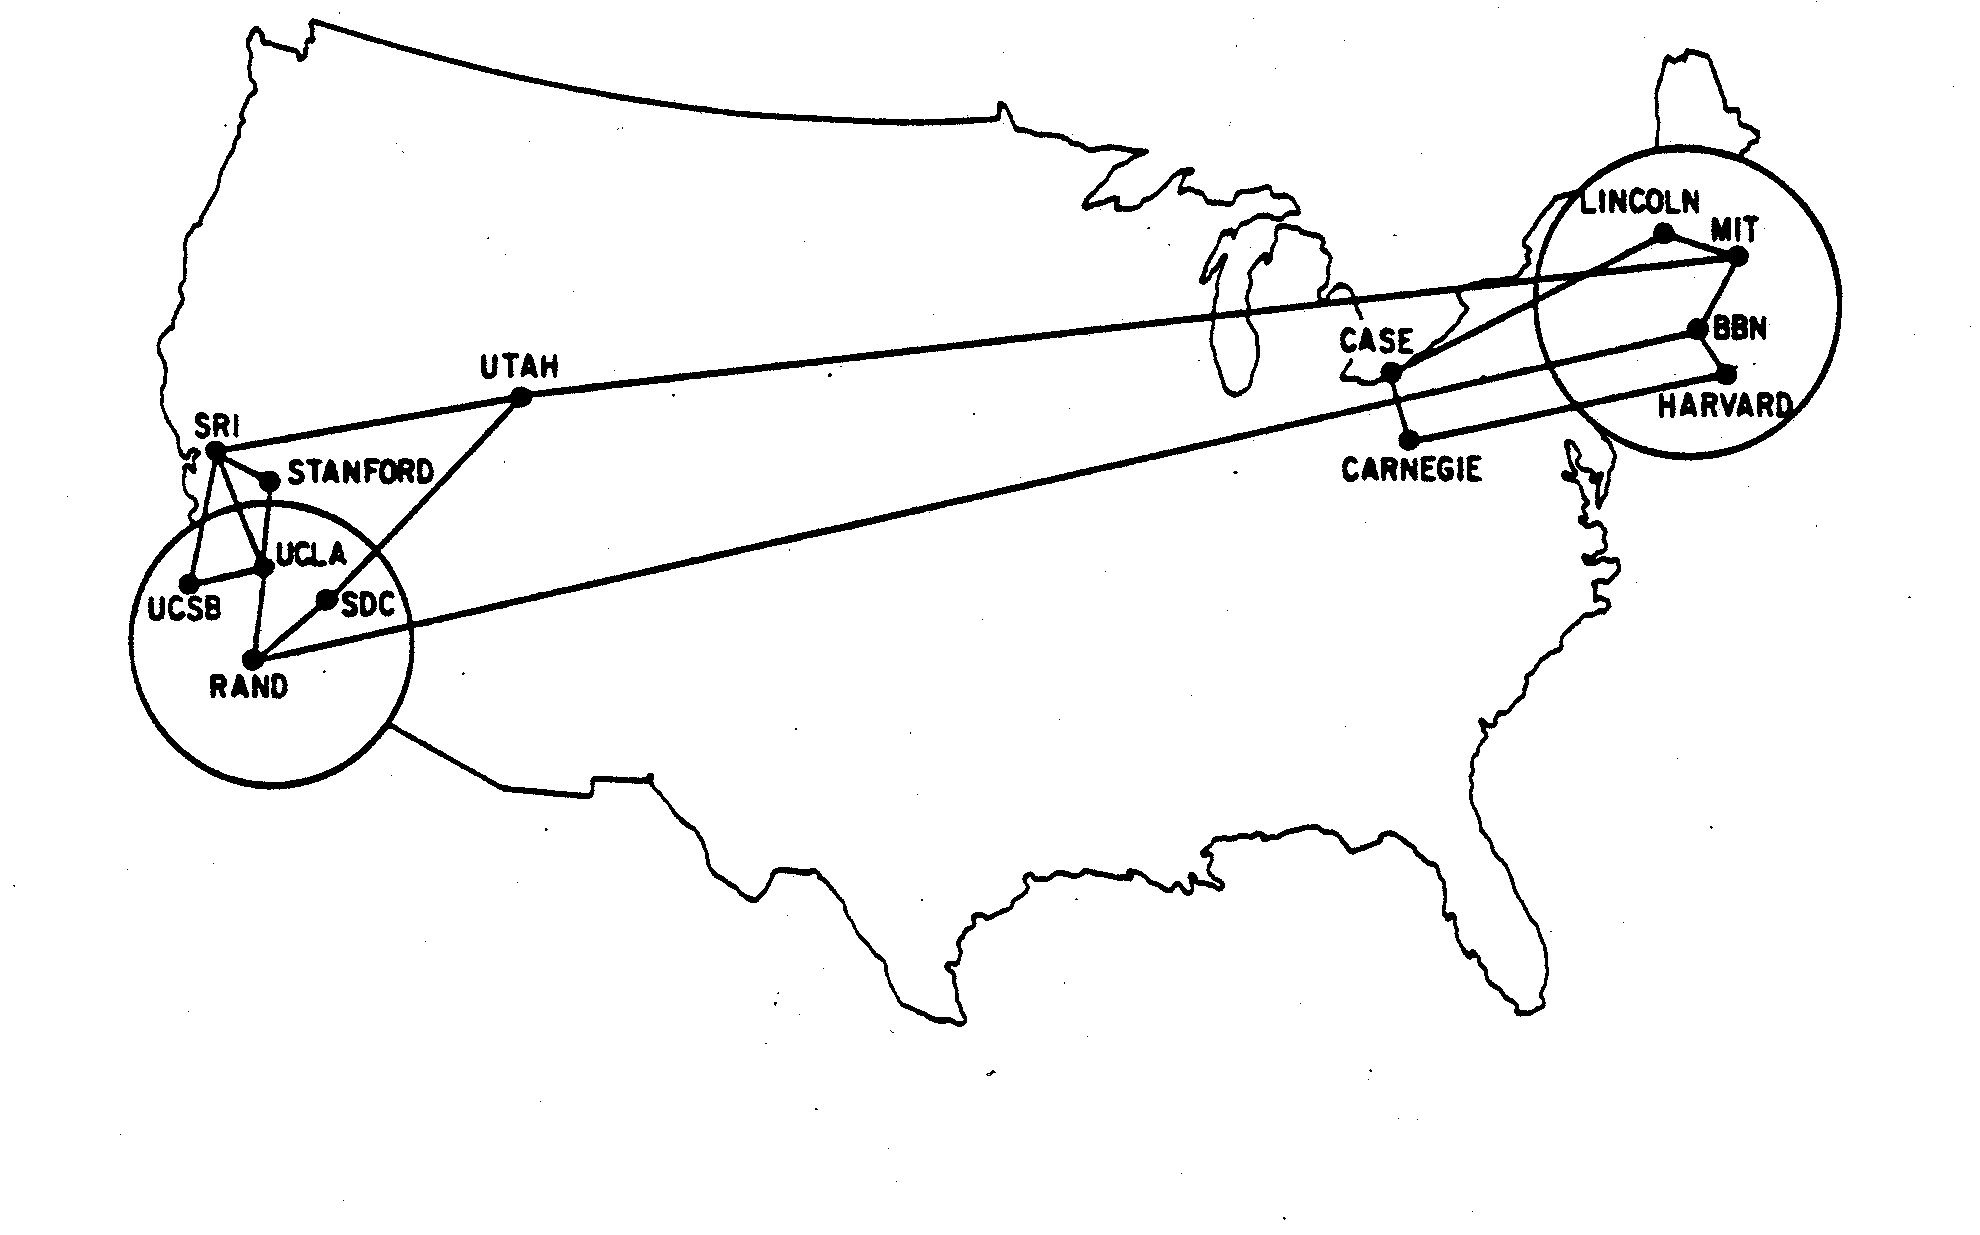
\includegraphics[width=0.7\textwidth]{./images/f7dec1970.jpg}
    \caption{
        The Internet (more precisely, ARPANET) in December 1970.
        Nodes are computers, connected by a link if they can directly communicate with each other.
        At the time, only 13 computers participated in that network.
    }
\end{figure}

\begin{code}
\begin{minted}[linenos, breaklines, frame=single]{text}
UCSB SRI UCLA
SRI UCLA STAN UTAH
UCLA STAN RAND
UTAH SDC MIT
RAND SDC BBN
MIT BBN LINC
BBN HARV
LINC CASE
HARV CARN
CASE CARN
\end{minted}
\caption{\texttt{arpa.adj}}
\end{code}

The following \textbf{diagram}, built from the adjacencies in \verb|arpa.adj|, contains the same information as in the above figure, without the distracting details of US geography;
this is actually an important point, as networks only reflect the \textbf{topology} of the object being studied.

\begin{code}
\begin{minted}[linenos, breaklines, frame=single]{python}
H = nx.read_adjlist("../data/arpa.adj")
opts = { "with_labels": True, "node_color": 'y' }
nx.draw(H, **opts)
\end{minted}
\caption{\texttt{arpa.adj}}
\end{code}

\begin{figure}[H]
    \centering
    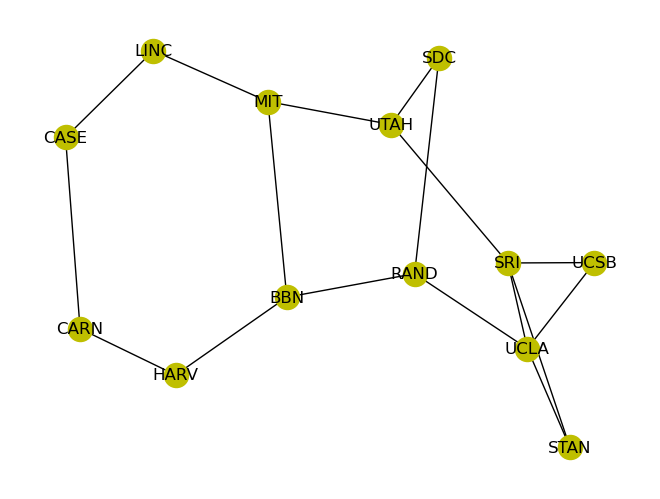
\includegraphics[width=0.7\textwidth]{./images/qwe_download.png}
    \caption{ The ARPA Network as a Graph }
\end{figure}

\subsection{Simple Graphs}
A \textbf{simple graph} is a pair $G = (X,E)$ consisting of a finite set $X$ of objects called \textit{nodes}, \textit{vertices}, or \textit{points} and a set of \textit{links} or \textit{edges} $E$ which are each a set of two different vertices. 
\begin{itemize}
    \item   We can also write $E \subseteq \binom{X}{2}$, where $\binom{X}{2}$ ($X$ \textit{choose} 2) is the set of all $2$-element subsets of $X$.
    \item   The \textbf{order} of the graph $G$ is denoted as $n = |X|$, where $n$ is the number of vertices in the graph.
    \item   The \textbf{size} of the graph is denoted as $m = |E|$, where $m$ is the number of edges in the graph.
            Naturally, $m \leq \binom{n}{2}$.
\end{itemize}

\subsubsection{Example}
$G=(X,E)$ with $X = \{ A, B, C, D \}$ and $E = \{ \{AB\}, \{BC\}, \{BD\}, \{CD\} \}$, so $G$ is a graph of order $4$ and size $4$.
We can be lazy and write $\{ A, B \}$ as just $AB$, so $E = \{ AB, BC, BD, CD \}$.

\subsection{\mintinline{python}{networkx}}

\end{document}
